\chapter{Algorytm łączenia segmentów}

Niezależnie od formatu zapisu plików indeksu, łączenie segmentów odbywa się według tego samego algorytmu. Za proces ten odpowiedzialna jest metoda \texttt{merge()} klasy \texttt{SegmentMerger} (klasa ta nie jest widoczna poza swoim pakietem -- nie można jej nadpisać ani rozszerzyć w implementacji swojego kodeka). Oto kolejność łączenia poszczególnych elementów segmentu:
\begin{enumerate}
 \item łączenie \texttt{FieldInfos},
 \item łączenie \texttt{Fields},
 \item łączenie \texttt{Terms}: łączenie list postingowych przypisanych do termów,
 \item łączenie \texttt{DocValues} (o ile zostały zaindeksowane),
 \item łączenie norm (o ile zostały zaindeksowane),
 \item łączenie \texttt{TermVectors} (o ile zostały zaindeksowane).
\end{enumerate}

%\section{Algorytm łączenia termów}
%
Łączenie termów i następujące w związku z nim łączenie list postingowych jest najważniejszym elementem całego procesu. Przyjrzymy mu się dokładniej.

Cały proces przebiega rekurencyjnie, po strukturze indeksu przedstawionej na rys. \ref{fig:indexApi}. Oznacza to, że najpierw łączone są definicje pól w obrębie zbioru łączonych segmentów. Jeśli dane pole występuje w więcej niż jednym segmencie, to w jego obrębie łączone są wszystkie termy. Analogicznie, jeśli w dwóch segmentach występuje ten sam term we właśnie połączonym polu, łączone są listy postingowe dla tego termu.

\section{Łączenie pól}

Algorytm łączenia pól pochodzących z różnych segmentów ilustruje rys. \ref{fig:fieldMerge}. Dla każdego z łączonych segmentów pobrany jest \texttt{AtomicReader}. Na jego podstawie utworzona zostaje instancja klasy \texttt{ReaderSlice}, przechowująca następujące informacje:
\begin{enumerate}
 \item \texttt{docBase}: pierwszy numer, jaki zostanie nadany dokumentowi pochodzącego z obecnego \texttt{AtomicReadera} i zapisanego w wynikowym segmencie. W obrębie jednego segmentu numery dokumentów (\emph{docId}) są unikalne i zaczynają się od 0. W związku z tym podczas łączenia dokumenty z co najmniej jednego segmentu muszą zostać przenumerowane. Do tego właśnie służy \texttt{docBase}: zostanie ona dodana do wszystkich \emph{docId} danego segmentu. Wartość \texttt{docBase} dla pierwszego z łączonych segmentów wynosi 0, dla każdego kolejnego jest równa łącznej liczbie dokumentów z poprzednich segmentów;
 \item \texttt{maxDoc}: liczba dokumentów zaindeksowanych w danym segmencie;
 \item \texttt{readerIndex}: numer porządkowy segmentu.
\end{enumerate}

Z każdego \texttt{AtomicReadera} pobrana jest także instancja \texttt{Fields}. Tablice z odpowiadającymi sobie instancjami \texttt{ReaderSlice} oraz \texttt{Fields} służą do zainicjalizowania klasy \texttt{MultiFields}, służącej jako agregat pól.

\begin{figure}[here]
 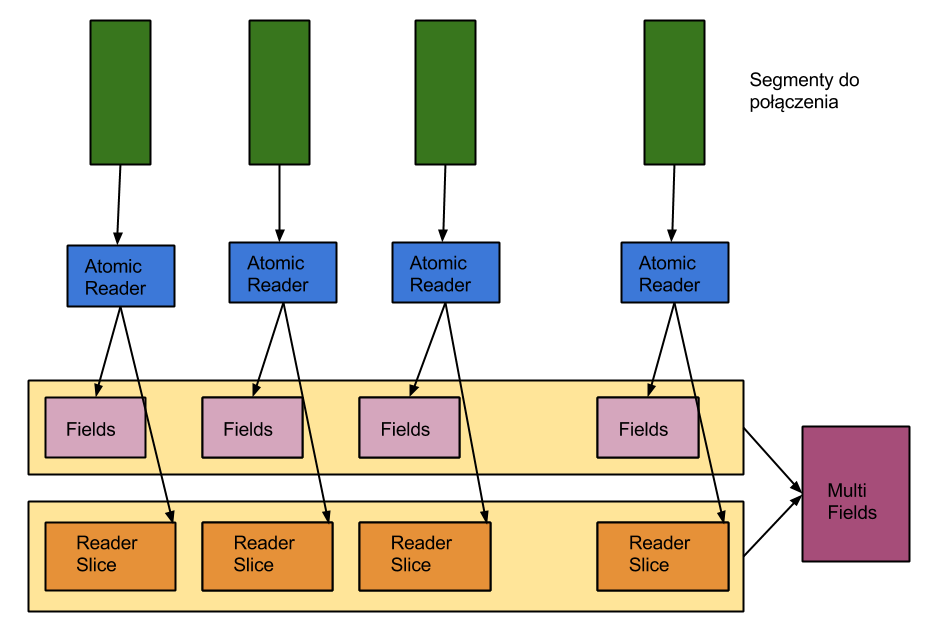
\includegraphics[scale=0.4]{pictures/LaczeniePol.png}
 \caption{Schematyczne ujęcie procesu łączenia pól z różnych segmentów. Źródło: opracowanie własne. \label{fig:fieldMerge}}
\end{figure}

\section{\texttt{MultiFields}}

\texttt{MultiFields} jest rozszerzeniem klasy \texttt{Fields}. Grupuje w sobie reprezentacje pól pochodzących z różnych segmentów i pozwala na operowanie ich zawartością tak, jakby były to pola pobrane z jednego segmentu. Jego schemat (oraz schematy klas powiązanych) przedstawia rys. \ref{multiFields}.

\begin{figure}[here]
 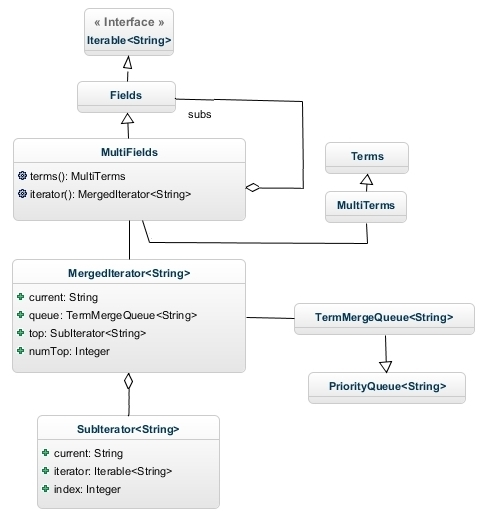
\includegraphics[scale=0.65]{pictures/MultiFields_2.jpg}
 \caption{\texttt{MultiFields} oraz klasy powiązane. Źródło: opracowanie własne.\label{multiFields}}
\end{figure}

To, że \texttt{MultiFields} jest rozszerzeniem klasy \texttt{Fields} oznacza, że posiada wszystkie jej funkcjonalności i w ich obrębie posługuje się takim samym interfejsem. Z punktu widzenia klasy zarządzającej procesem łączenia segmentów (\texttt{SegmentMergera}) zachowuje się więc dokładnie jak \texttt{Fields}. Jest to przykład dobrego podziału odpowiedzialności pomiędzy klasami i ukrywania wewnętrznej implementacji.

Z punktu widzenia algorytmu łączenia segmentów, najbardziej interesującymi metodami \texttt{MultiFields} są \texttt{MultiFields.terms(String field)}, zwracająca termy należące do pola o podanej nazwie oraz \texttt{MultiFields.iterator()}, zwracająca iterator pozwalający na przechodzenie po kolejnych nazwach pól. 

\section{\texttt{MultiFields.terms()}}

\texttt{MultiFields.terms()} zwraca instancję typu \texttt{MultiTerms}. Podobnie jak \texttt{MultiFields} agreguje pola z różnych segmentów, ale zachowuje się tak, jak \texttt{Fields} pochodzące z pojedynczego segmentu, tak \texttt{MultiTerms}  gromadzi wszystkie termy znajdujące się w danym polu. Ukrywa też to, że dla danego termu być może mamy do czynienia z kilkoma termami o takim samym tokenie, ale pochodzącymi z tego samego pola z różnych segmentów.

Schemat tworzenia instancji \texttt{MultiTerms} znajduje się na rys. \ref{fig:multiTerms}. Nietrudno dostrzec podobieństwo z algorytmem tworzenia instancji \texttt{MultiFields} (rys. \ref{fig:fieldMerge}). Instancje \texttt{Terms} są pobrane przy pomocy \texttt{Fields.terms(f)} dla \texttt{f} będącego nazwą pola. Jeśli obiekt \texttt{Terms} istnieje dla danego pola (tzn. \texttt{terms(f) != null}), podawany jest, wraz z odpowiadającym mu obiektem \texttt{ReaderSlice}, do właśnie tworzonej instancji \texttt{MultiTerms}.

\begin{figure}[here]
 \centering
 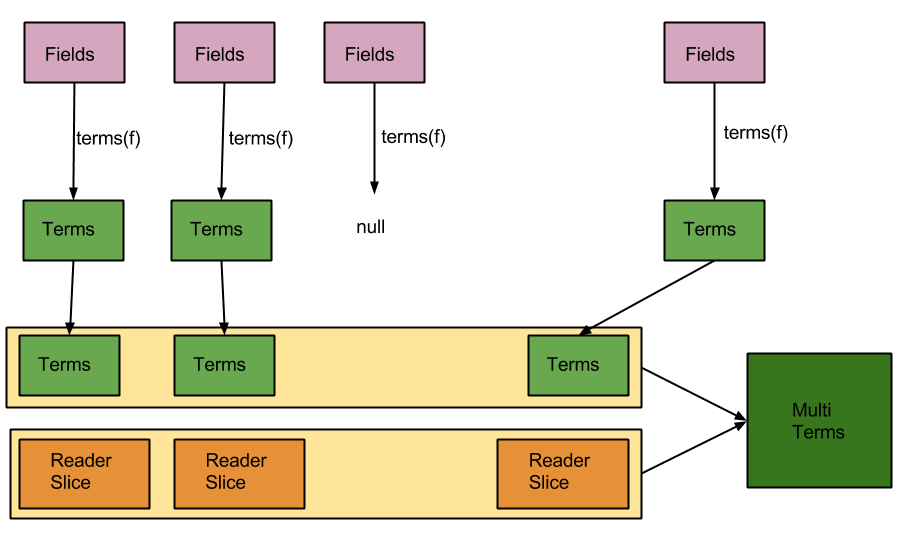
\includegraphics[scale=0.4]{pictures/MultiTerms.png}
 \caption{Schemat tworzenia instancji \texttt{MultiTerms}. Źródło: opracowanie własne. \label{fig:multiTerms}}
\end{figure}

\section{\texttt{MultiFields.iterator()}}

Jak zostało to już wspomniane, \texttt{Fields.iterator()} przechodzi po nazwach pól zgromadzonych w klasie \texttt{Fields}. Kolejne elementy zwracane przez ten iterator są uporządkowane rosnąco. \texttt{MultiFields.iterator()}, aby spełnić to wymaganie, posługuje się własną implementacją iteratora napisów -- klasą \texttt{MergedIterator}. Oto jej specyfikacja:
\begin{itemize}
 \item \texttt{MergedIterator} jest tworzony na podstawie iteratorów napisów $i_1$, $i_2$, ... $i_n$. Zwraca kolejno elementy tych iteratorów posortowane rosnąco; 
 \item jeśli dany element występuje w więcej niż jednym z iteratorów $i_1$, $i_2$, ... $i_n$, \texttt{MergedIterator} zwraca go tylko raz.
\end{itemize}
Iteratory $i_1$, $i_2$, ... $i_n$ pochodzą z instancji \texttt{Fields} zgromadzonych w \texttt{MultiFields}. \texttt{MergedIterator} wykorzystuje kolejkę priorytetową do przechowywania zagregowanych iteratorów. Porządek kolejki jest zdefiniowany przez elementy, na które w danym momencie wskazują iteratory $i_k, k \in \{1, ..., n\}$.

\section{Łączenie termów}

Łączenie termów odbywa się w metodzie \texttt{merge()} klasy \texttt{TermsConsumer}, która jako parametry przyjmuje:
\begin{itemize}
 \item \texttt{MergeState} -- pomocniczy obiekt przechowujący stan obecnego procesu łączenia segmentów. Gromadzi listę \texttt{AtomicReaderów}, strukturę z informacją o dokumentach do usunięcia, itp. Nie będziemy się nim zajmować w dalszej części pracy;
 \item \texttt{IndexOptions} -- wartość wskazująca na to, jakie informacje o termach i ich wystąpieniach zostały zaindeksowane. \texttt{IndexOptions} przyjmuje jedną z czterech wartości:
 \begin{enumerate}
  \item \texttt{DOCS\_ONLY}: oznacza, że w indeksie znajduje się tylko informacja o tym, czy dany term tam wystąpił, czy nie. Częstości występowania termu oraz pozycje wystąpień są pominięte -- co skutkuje np. tym, że zapytania frazowe nie mogą zostać na takim indeksie wykonane. Obliczanie zgodności zapytania z dokumentem zachowuje się tak, jakby każdy term występował w dokumencie dokładnie raz.
  \item \texttt{DOCS\_AND\_FREQS}: dla każdego termu zapamiętana jest informacja o jego liczbie wystąpień w dokumencie. Dzięki temu podobieństwo zapytania do dokumentu może być obliczone precyzyjniej. Zapytania frazowe oraz inne, wykorzystujące informacje o pozycjach termów, nie mogą być wykonywane.
  \item \texttt{DOCS\_AND\_FREQS\_AND\_POSITIONS}: najczęściej wykorzystywany sposób indeksowania: w indeksie pamiętane są częstości termów oraz pozycje ich wystąpień, w związku z czym możliwe jest wykonywanie wielu typów zapytań.
  \item \texttt{DOCS\_AND\_FREQS\_AND\_POSITIONS\_AND\_OFFSETS}: poza częstościami i pozycjami wystąpień termów pamiętane są informacje o dokładnym położeniu każdego termu (tzn. odległości znakowej od początku dokumentu) i jego faktycznej długości (pamiętamy o tym, że różne formy danego termu podczas analizy są sprowadzane do formy bazowej -- dlatego informacja o pierwotnej długości wystąpienia musi być dodatkowo zapamiętywana).
 \end{enumerate}
 \item \texttt{TermsEnum} -- w procesie łączenia termów będzie to instancja \texttt{MultiTermsEnum}, pobrana z obiektu \texttt{MultiTerms}.
\end{itemize}

W najprostszym przypadku -- dla opcji \texttt{DOCS\_ONLY} -- algorytm łączenia termów wygląda następująco:
\begin{enumerate}
 \item Zainicjalizuj zbiór dokumentów odwiedzonych już dla właśnie łączonego termu (\texttt{visitedDocs}).
 \item Zainicjalizuj pole \texttt{docsEnum} typu \texttt{MappingMultiDocsEnum}, o ile nie zostało to jeszcze zrobione (leniwa inicjalizacja -- właśnie łączony term jest pierwszym z termów pola).
 \item Dla każdego termu \texttt{t} dostępnego z \texttt{MultiTermsEnum} pobierz listę \texttt{docsEnumIn} dokumentów, w których term ten występuje. Lista opakowana jest w instancję klasy \texttt{MultiDocsEnum}. Dodaj dokumenty z \texttt{docsEnumIn} do \texttt{docsEnum}. Wykonaj kroki \ref{enum:begin} -- \ref{enum:end} dla \texttt{t}.
 \item \label{enum:begin} Rozpocznij zapis listy postingowej dla \texttt{t} (przy pomocy wywołania \texttt{startTerm(t)}). Jednocześnie pobierz instancję \texttt{PostingsConsumera}, która umożliwi połączenie list postingowych pochodzących z różnych segmentów.
 \item Wywołaj \texttt{PostingsConsumer.merge()}, jako parametry przekazując obiekt przechowujący stan, \texttt{DOCS\_ONLY} jako opcję indeksowania, \texttt{docsEnum} i listę odwiedzonych już dokumentów.
 \item \label{enum:end} Zakończ zapis termu (\texttt{PostingsConsumer.finishTerm()}), zapamiętaj liczbę dokumentów w połączonej liście.
\end{enumerate}

Dla pozostałych wartości parametru \texttt{IndexOptions} łączenie termów przebiega podobnie. Różni się jedynie typami struktur przechowujących referencje do list postingowych.
\begin{itemize}
 \item W przypadku \texttt{DOCS\_AND\_FREQS} korzystamy z innej instancji typu \texttt{MappingMultiDocsEnum}, \texttt{docsAndFreqsEnum}, zamiast \texttt{docsEnum}.
 \item W przypadkach \texttt{DOCS\_AND\_FREQS\_AND\_POSITIONS} i \texttt{DOCS\_AND\_FREQS\_AND\_POSITIONS\_AND\_OFFSETS} korzystamy z tej samej instancji klasy \texttt{MappingMultiDocsAndPositionsEnum}, \texttt{postingsEnum}.
\end{itemize}
Różne typy i różne instancje przechowujące dane o listach postingowych są tutaj potrzebne, ponieważ w ramach jednego procesu łączenia segmentów możemy mieć do czynienia z różnymi opcjami indeksowania pól (jak już wspomniano, opcje indeksowania pól są całkowicie od siebie niezależne, nawet dla pól występujących w tym samym segmencie).

\section{Łączenie list postingowych}

Łączenie list postingowych jest zaimplementowane w metodzie \texttt{merge()} klasy \texttt{PostingsConsumer}. Metoda ta przyjmuje następujące parametry, przekazywane z \texttt{TermsConsumer.merge()}:
\begin{itemize}
 \item \texttt{MergeState}: tutaj niepotrzebny, nigdzie nie używany. Prawdopodobnie jest to pozostałość po starej implementacji i zostanie usunięta w najbliższym czasie.
 \item \texttt{IndexOptions}: podobnie, jak w przypadku łączenia termów, dokładny algorytm zależy od wybranej opcji indeksowania.
 \item \texttt{DocsEnum}: reprezentacja list dokumentów, które mają być połączone. Obecny kodek wykorzystuje \texttt{MappingMultiDocsEnum} lub \texttt{MappingMultiDocsAndPositionsEnum}, w zależności od opcji indeksowania (i instancji przekazanej tutaj z \texttt{TermsConsumer.merge()}). 
 \item \texttt{FixedBitSet}: zbiór bitowy reprezentujący odwiedzone już dokumenty.
\end{itemize}

Podobnie, jak w \texttt{TermsConsumer.merge()} opcje indeksowania wpływają na algorytm łączenia list. W najprostszym przypadku (dla \texttt{IndexOptions.DOCS\_ONLY}) algorytm ten ma następujący przebieg:
\begin{enumerate}
 \item \label{jeden} Pobierz kolejny posting z listy (z \texttt{DocsEnum}) do zmiennej \texttt{doc}. Jeśli otrzymaną wartością jest \texttt{NO\_MORE\_DOCS}, zakończ algorytm. W przeciwnym wypadku przejdź do kroku \ref{dwa}.
 \item \label{dwa} Zaznacz \texttt{doc} jako odwiedzony (skorzystaj z dostarczonej instancji \texttt{FixedBitSet}).
 \item \label{trzy} Rozpocznij zapis postingu. Wpisz wartość \texttt{doc}.
 \item Zakończ zapis postingu.
 \item Przejdź do kroku \ref{jeden}.
\end{enumerate}

W przypadku innych opcji indeksowania do powyższego algorytmu wprowadza się kilka zmian.
\begin{itemize}
 \item Dla opcji \texttt{DOCS\_AND\_FREQS}, poza pobraniem postingu z listy \texttt{DocEnum} w kroku \ref{jeden}, odczytuje się także częstość występowania termu w dokumencie, \texttt{docFreq}, która później zapisywana jest wraz z postingiem w kroku \ref{trzy}.
 \item Dla opcji \texttt{DOCS\_AND\_FREQS\_AND\_POSITIONS} dodatkowo odczytywane są (i później zapisywane do listy wynikowej) pozycje wystąpień termu w dokumencie oraz ewentualne \emph{payloads}, a dla \texttt{DOCS\_AND\_FREQS\_AND\_POSITIONS\_AND\_OFFSETS} -- również ich odległości znakowe od początku dokumentu i długości.
\end{itemize}

\section{Rozszerzenia klasy \texttt{DocsEnum} używane w procesie łączenia postingów}

\texttt{DocsEnum} jest abstrakcją pozwalającą pobierać kolejne elementy list postingowych. Jej interfejs zawiera jedynie metody zwracające numer dokumentu obecnie wskazywanego przez iterator, jego częstość oraz pozwalające na przejście do kolejnych dokumentu. Dodatkowe funkcjonalności są implementowane przez jej liczne rozszerzenia (np. wspomniany już \texttt{DocsAndPostitionsEnum}). W algorytmie łączenia list postingowych wykorzystywane są cztery z nich: \texttt{MultiDocsEnum}, \texttt{MappingMultiDocsEnum} oraz odpowiadające im \texttt{MultiDocsAndPositionsEnum} i \texttt{MappingMultiDocsAndPositionsEnum}. Przyjrzymy się im dokładniej.

Podczas łączenia termów (w metodzie \texttt{TermsConsumer.merge()}) z iteratora termów (konkretniej: z instancji \texttt{MultiTermsEnum}) pobierany jest obiekt \texttt{MultiDocsEnum}. Zawiera on informacje o listach postingowych dla danego termu pochodzących z łączonych segmentów oraz odpowiadające im wskaźniki na dany segment (w postaci obiektów \texttt{ReaderSlice}). Schemat klasy \texttt{MultiDocsEnum} przedstawia rys. \ref{fig:multiDocsEnum}.

\begin{figure}[here]
 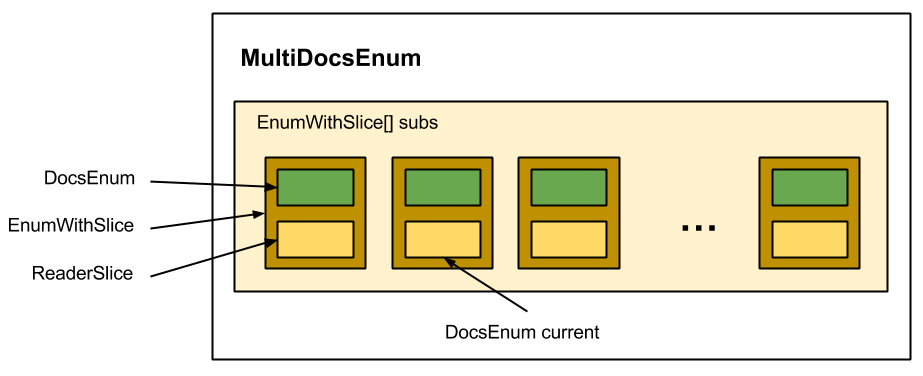
\includegraphics[scale=0.4]{pictures/MultiDocsEnum.png}
 \caption{\texttt{MultiDocsEnum} i jej zawartość. Źródło: opracowanie własne. \label{fig:multiDocsEnum}}
\end{figure}

Poza innymi wskaźnikami i zmiennymi, \texttt{MultiDocsEnum} posługuje się zmienną \texttt{current} wskazującą na obecnie odczytywany iterator dokumentów -- \texttt{current} odwiedza wszystkie zgromadzone obiekty \texttt{DocsEnum} i iteruje po ich zawartości. Przeskakuje na następny w momencie wyczerpania postingów w obecnie odwiedzanej instancji \texttt{DocsEnum}. Dzięki temu z punktu widzenia klasy \texttt{PostingsConsumer} \texttt{MultiDocsEnum} zachowuje się dokładnie tak samo, jak każdy \texttt{DocsEnum}. 

Obiekty \texttt{ReaderSlice} służą z kolei do odczytywania podstawy przenumerowania dokumentów pochodzących z danego segmentu.

\texttt{MappingMultiDocsEnum}, poza wymienionymi wyżej strukturami, zawiera także infomację o tym, które dokumenty powinny zostać usunięte podczas łączenia segmentów. Jest ona przechowywana w strukturze \texttt{DocMap} i pobierana jest z instancji \texttt{MergeState} (rys. \ref{fig:mappingMultiDocsEnum}). Instancja \texttt{MappingMultiDocsEnum} jest tworzona podczas łączenia termów w metodzie \texttt{TermsConsumer.merge()} -- listy postingowe z pobranego wcześniej obiektu \texttt{MultiDocsEnum} są do niej kopiowane i w dalszej części algorytmu wszystkie operacje na tych listach wykonywane są właśnie na kopiach znajdujących się w \texttt{MappingMultiDocsEnum}. 

Celem tego zabiegu jest zachowanie podzielonej odpowiedzialności: zadaniem \texttt{MultiDocsEnum} jest gromadzenie kilku \texttt{DocsEnum} i przedstawianie ich w postaci jednego iteratora. \texttt{MappingMultiDocsEnum} natomiast do tych funkcjonalności dodaje jeszcze możliwość pomijania dokumentów gotowych do usunięcia z indeksu. 

\begin{figure}[here]
 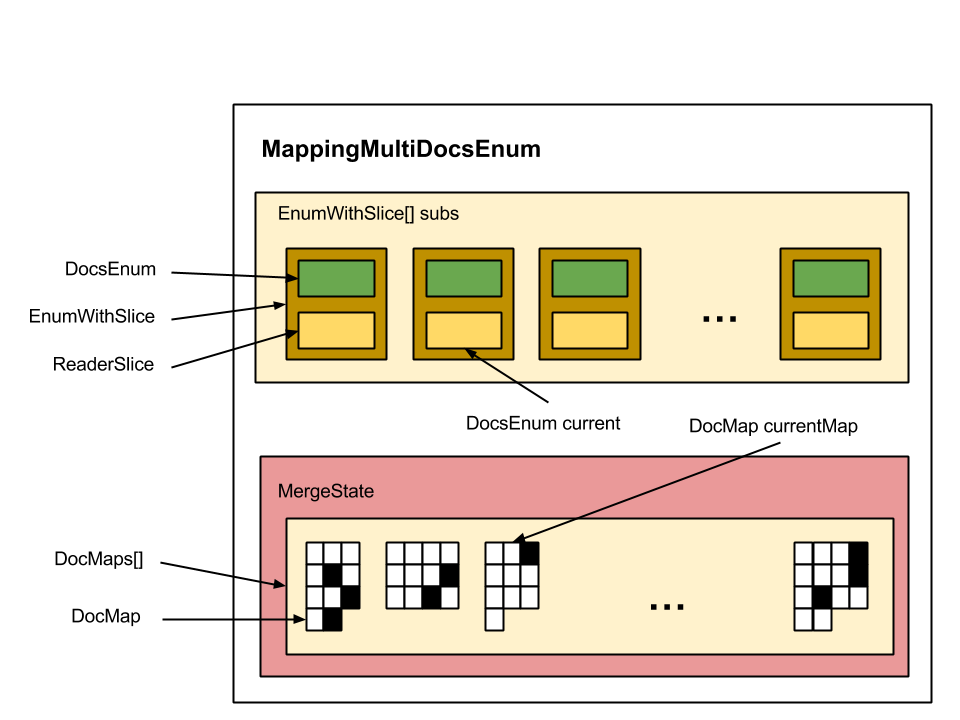
\includegraphics[scale=0.4]{pictures/MappingMultiDocsEnum.png}
 \caption{\texttt{MappingMultiDocsEnum}. Źródło: opracowanie własne. \label{fig:mappingMultiDocsEnum}}
\end{figure}

Gdy \texttt{MappingMultiDocsEnum} pytany jest o kolejny dokument z właśnie rozpatrywanej listy postingowej, sprawdza najpierw w odpowiedniej instancji \texttt{DocMap}, czy kolejny wskazywany dokument na liście jest ,,żywy''. Podaje jego numer tylko wtedy, jeśli faktycznie tak jest. W ten sposób dokumenty zaznaczone do usunięcia są pomijane w procesie łączenia list. 

Przepisywanie zawartości jednej klasy do drugiej nie jest najelegantszym rozwiązaniem -- z punktu widzenia czystości kodu lepsze byłoby tutaj zastosowanie wzorca projektowego \emph{dekorator}: \texttt{MappingMultiDocsEnum} mógłby opakowywać instancję \texttt{MultiDocsEnum} i jednocześnie rozszerzać funkcjonalność \texttt{DocsEnum} o pomijanie dokumentów gotowych do usunięcia.

\section{Propozycja optymalizacji algorytmu łączenia list postingowych}

\subsection{Opis problemu}

Zauważmy, że w procesie łączenia list postingowych numery dokumentów przepisywane są pojedynczo: dowolne rozszerzenie \texttt{DocsEnum} potrafi podawać kolejne postingi, jeden za drugim, bez możliwości ich grupowania. Listy postingowe w plikach indeksu trzymane są w formie zakodowanej (por. \ref{sec:packedBlockEncoding} i \ref{sec:vIntEncoding}), natomiast numery dokumentów gotowych do usunięcia są (w uproszczeniu) dostępne jako liczby całkowite. W związku z tym, podczas łączenia list postingowych każdy posting musi być odkodowany w celu sprawdzenia, czy ma on być zapisany do listy wynikowej, czy nie. Jeśli dany dokument jest ,,żywy'' (nie znajduje się na liście dokumentów do usunięcia), jego numer musi zostać ponownie zakodowany przed zapisaniem. Zatem dla list postingowych długości $l_1$ i $l_2$ wykonujemy $O(l_1 + l_2)$ operacji odkodowania i zakodowania liczby całkowitej.

W większości systemów wyszukiwania dokumenty usuwane są dość rzadko -- co oznacza, że w ogólnym przypadku liczba ,,martwych'' postingów w łączonych listach jest stosunkowo mała. W związku z tym często możnaby unikać niepotrzebnych operacji kodowania i odkodowania. Wymaga to jednak modyfikacji algorytmu łączenia list: chcielibyśmy móc niekiedy kopiować całe zakodowane bloki zamiast pojedynyczych postingów. Pomysł taki został zgłoszony w systemie zarządzania zadaniami związanym z Lucene (Lucene Jira, \cite{jira}). Jego skrótowy opis znajduje się w \cite{idea}.

Blok postingów mógłby zostać przekopiowany bez dekodowania, o ile liczba dokumentów usuniętych znajdujących się w nim byłaby stosunkowo mała (implementacja rozwiązania zawierałaby modyfikowalną maksymalną dopuszczalną liczbę ,,martwych'' dokumentów w bloku). Jeśli w danym bloku byłoby więcej dokumentów do usunięcia, byłby on przepisywany tak, jak dotychczas -- po jednym elemencie.

\subsection{Proponowane rozwiązanie}
\label{sec:solution}

W tej sekcji omówione zostanie proponowane rozwiązanie dla najprostszego przypadku indeksowania (\texttt{IndexOptions.DOCS\_ONLY}). Wprowadzenie opisanej wyżej modyfikacji wymaga rozwiązania dwóch problemów:
\begin{enumerate}
 \item w jaki sposób zmienić architekturę części odpowiadającej za łączenie list postingowych tak, aby istniała możliwość kopiowania zarówno bloków (bez dekodowania) oraz pojedynczych postingów?
 \item jak wyznaczyć bloki gotowe do przekopiowania?
\end{enumerate}

Zmiany w architekturze rozpoczynają się od wprowadzenia klasy reprezentującej element listy postingowej, \texttt{PostingElement}. Jej schemat specyfikuje rys. \ref{fig:postingElement}. W zależności od tego, jaki fragment listy postingowej jest zwracany (\texttt{type} przyjmujące wartość \texttt{PostingElementType.BLOCK} lub \texttt{PostingElementType.INT}), inicjalizowane jest pole \texttt{postingBlocks} lub \texttt{posting}.

\begin{figure}[here]
 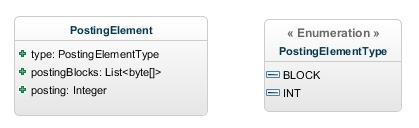
\includegraphics[scale=0.7]{pictures/PostingElement.jpg}
 \caption{Klasa \texttt{PostingElement}. Źródło: opracowanie własne. \label{fig:postingElement}}
\end{figure}

Dodatkowo, potrzebne są też odpowiedniki klas \texttt{DocsEnum} oraz \texttt{MultiDocsEnum} potrafiące się nią posługiwać. Wprowadzamy więc \texttt{PostingElementEnum} oraz \texttt{MultiPostingElementEnum} (rys. \ref{fig:postingEnums}).

\begin{figure}[here]
 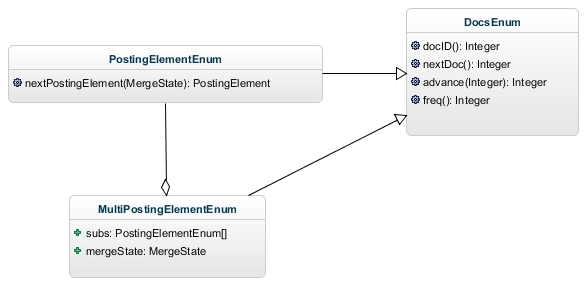
\includegraphics[scale=0.7]{pictures/PostingEnums.jpg}
 \caption{\texttt{PostingElementEnum} oraz \texttt{MultiPostingElementEnum} -- rozszerzenia \texttt{DocsEnum} wykorzystywane w zmodyfikowanym algorytmie łączenia list postingowych. Źródło: opracowanie własne. \label{fig:postingEnums}}
\end{figure}

Taka zmiana wymaga uzasadnienia kilku kwestii.
\begin{enumerate}
 \item \label{item:inheritance} Jak można odczytać z diagramu \ref{fig:postingEnums}, zarówno \texttt{PostingElementEnum} oraz \texttt{MultiDocsAndPositionsEnum} rozszerzają klasę \texttt{DocsEnum} i w związku z tym dziedziczą jej interfejs, posługujący się jedynie liczbami całkowitymi. Na pierwszy rzut oka może to wydawać się niezgodne z ideą zmiany -- chcemy wszak wprowadzić abstrakcję opakowującą elementy list postingowych (do tego służy nam właśnie \texttt{PostingElement}) i nowe klasy powinny się tylko nią posługiwać. Dziedziczenie po \texttt{DocsEnum} służy tutaj zachowaniu zgodności z resztą systemu -- chcemy, aby wprowadzone zmiany jak najmniej modyfikowały istniejący interfejs programisty biblioteki i jak najmniej ingerowały w strukturę klas -- w szczególności, jeśli nie są to klasy pojedynczego kodeka, a klasy wspólne, wykorzystywane przez wszystkie kodeki. Dodatkowo, dziedziczenie po \texttt{DocsEnum} pozwoli nam wykorzystać to, że lista postingowa jest skip listą (co okaże się przydatne podczas wyznaczania fragmentu listy do późniejszego przekopiowania).
 \item Wszystkie metody klasy \texttt{DocsEnum} są abstrakcyjne. W związku z tym, dużo bardziej elegancko byłoby posłużyć się w tym wypadku interfejsem (najlepiej parametryzowanym), a nie klasą abstrakcyjną. Możnaby wtedy uprościć hierarchię iteratorów postingów dzięki wykorzystaniu wielodziedziczenia (w Javie klasy mogą dziedziczyć tylko po jednej klasie bazowej -- mogą natomiast implementować wiele interfejsów): funkcjonalność iterowania po postingach można byłoby wtedy oddzielić od funkcjonalności grupowania innych iteratorów. Taka zmiana wymagałaby jednak przebudowania znacznej części Lucene. Warto wspomnieć to, że \texttt{DocsEnum} dziedziczy implementację metody \texttt{slowAdvance(int target)} po \texttt{DocIdSetIteratorze}. Zatem przepisanie abstrakcyjnego \texttt{DocsEnum} na interfejs wymagałoby przeniesienia implementacji \texttt{slowAdvance()} w inne miejsce. Ponadto, zmiany tego typu prawdopodobnie nie poprawiłaby niczego poza czytelnością kodu. Praktycznie rzecz biorąc nie warto więc ich wprowadzać.
 \item W punkcie \ref{item:inheritance} jako jeden z argumentów za dziedziczeniem \texttt{PostingElementEnum} z \texttt{DocsEnum} wspomniane zostało współdzielenie operowania na liście postingowej jak na skip liście. Możnaby tutaj pokusić się o oddzielenie tego zadania od reszty funkcjonalności \texttt{DocsEnum} poprzez wyekstrahowanie interfejsu \texttt{Skippable}, gromadzącego metody \texttt{advance(int target)} i \texttt{slowAdvance(int target)}. Poprzez wprowadzenie relacji implementowania interfejsu pomiędzy \texttt{DocsEnum} i \texttt{Skippable} oraz \texttt{PostingElementEnum} i \texttt{Skippable}, zależność między \texttt{DocsEnum} i \texttt{PostingElementEnum} byłaby rozluźniona -- potencjalnie możnaby nawet zrezygnować z relacji dziedziczenia pomiędzy tymi klasami. Wadą takiego rozwiązania byłby brak możliwości dziedziczenia implementacji metody \texttt{slowAdvance()}, która w obecnym kształcie systemu jest taka sama dla wszystkich iteratorów elementów list postingowych.
\end{enumerate}

Wprowadzenie \texttt{PostingElement} oraz nowych iteratorów postingów wymagałoby też zmian w metodach \texttt{merge()} klas \texttt{TermsConsumer} oraz \texttt{PostingsConsumer}. Iterowanie po postingach i ich odczyt jest wykonywany przez \texttt{PostingElementEnum}, samo łączenie odbywa się w metodzie wspomnianej powyżej. Dodatkowo, \texttt{PostingsConsumer} (a dokładniej: jego rozszerzenie przypisane do danego kodeka) jest odpowiedzialny za zapis list postingowych. Należy zatem dodać mu funkcjonalność zapisu zakodowanych bloków postingów. 

Od strony implementacyjnej, najprostszym sposobem dodania wspomnianych funkcjonalności jest zastosowanie wzorca projektowego \emph{dekorator}: opakowanie klasy \texttt{PostingsConsumer} w klasę, która jednocześnie dziedziczyć będzie po niej zachowanie. Klasę opakowującą nazwijmy \texttt{BlockPostingsConsumer}. Jej nowe funkcjonalności są zaimplementowane bezpośrednio, natomiast fukcjonalności dziedziczone z \texttt{PostingsConsumer} są delegowane do wewnętrznej instancji tego typu. Metoda \texttt{merge()}, pochodząca z \texttt{PostingsConsumer} jest nadpisana w \texttt{BlockPostingsConsumer}.

\begin{figure}[here]
 \centering
 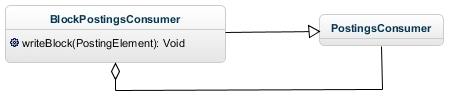
\includegraphics[scale=0.8]{pictures/PostingsConsumerWrapper.jpg}
 \caption{\texttt{BlockPostingsConsumer} -- dekorator dla \texttt{PostingsConsumera}. Źródło: opracowanie własne. \label{fig:postingsConsumerWrapper}}
\end{figure}

Samo utworzenie instancji \texttt{BlockPostingsConsumer} mogłoby się odbywać w \texttt{TermsConsumer.merge()}. Instancja odpowiedniego dla kodeka \texttt{PostingsConsumera} zaraz po pobraniu byłaby opakowywana w nowe funkcjonalności poprzez wstrzyknięcie jej do konstruktora klasy \texttt{BlockPostingsConsumer}.

Ponadto, w klasie \texttt{TermsConsumer} pole \texttt{docsEnum} powinno zmienić typ z \texttt{MappingMultiDocsEnum} na \texttt{MultiPostingElementEnum}.

Nowy algorytm łączenia termów (\texttt{TermsConsumer.merge()}), wykorzystujący wyżej opisane zmiany, wyglądałby więc następująco:
\begin{enumerate}
 \item Zainicjalizuj pole \texttt{docsEnum} typu \texttt{MultiPostingElementEnum}, o ile nie zostało to jeszcze zrobione.
 \item Dla każdego termu \texttt{t} dostępnego z \texttt{MultiTermsEnum} pobierz iterator \texttt{docsEnumIn} typu \texttt{MultiPostingElementEnum} (ponieważ podczas łączenia termów mamy listy postingowe pochodzące z różnych segmentów, wiemy, że pobrany iterator jest agregatorem innych iteratorów).
 \item Rozpocznij zapis listy postingowej dla \texttt{t} (przy pomocy wywołania \texttt{startTerm(t)}). Pobierz instancję \texttt{PostingsConsumera}, i podaj ją jako parametr konstruktora klasy \texttt{BlockPostingsConsumer}.
 \item Wywołaj \texttt{BlockPostingsConsumer.merge()} z odpowiednimi parametrami (instancją \texttt{MergeState}, flagą opcji indeksowania oraz zmienną \texttt{docsEnumIn}).
 \item Zakończ zapis termu (\texttt{BlockPostingsConsumer.finishTerm()}).
\end{enumerate}

Jak widać, za łączenie postingów jest teraz odpowiedzialna klasa \texttt{BlockPostingsConsumer}. Oto szkic algorytmu łączenia list, do zaimplementowania w \texttt{BlockPostingsConsumer.merge()}. Metoda ta powinna przyjmować następujące parametry: \texttt{MergeState mergeState}, \texttt{IndexOptions indexOptions} i \texttt{PostingElementEnum postingsElementEnum}.
\begin{enumerate}
 \item Tak długo jak \texttt{postingsElementEnum} jest niepusty, wykonuj kroki \ref{newMergeBegin} -- \ref{newMergeEnd}.
 \item \label{newMergeBegin} Do zmiennej \texttt{posting} pobierz kolejny \texttt{PostingElement} z \texttt{postingsElementEnum}.
 \item \label{newMergeEnd} Jeśli \texttt{posting} jest typu \texttt{PostingElementType.BLOCK}, zapisz cały blok (lub bloki) przy pomocy \texttt{BlockPostingsConsumer.writeBlocks(posting.getBlocks())}. Jeśli \texttt{posting} jest typu \texttt{PostingElementType.INT}, skorzystaj ze ,,starego'' sposobu zapisu pojedynczego postingu (\texttt{PostingsConsumer.startTerm()}, \texttt{PostingsConsumer.finishTerm()}).
 \item Zakończ algorytm.
\end{enumerate}

Do rozwiązania pozostaje jeszcze następująca kwestia: jak ustalić, który fragment listy postingowej (pojedyncza wartość, pojedynczy blok, wiele bloków) powinien zostać przekopiowany? Klasą, która powinna o tym decydować będzie \texttt{PostingElementEnum} lub klasa z niej wywiedziona. 

Pomimo, że wszystkie bloki list postignowych są zakodowane i nie możemy pobrać z nich wartości bezpośrednio, możemy wykorzystać tzw. \texttt{skipData}. Pamiętamy, że lista postingowa jest skip listą. Przed każdym blokiem postingów zapisywana jest informacja o wskaźnikach do tego bloku oraz (odkodowana) wartość pierwszego elementu bloku. Mając dany \texttt{mergeState}, potrafimy wylistować numery wszystkich dokumentów usuniętych. Możemy więc ustalić (posługując się skip listą), jak o wiele bloków odległy jest kolejny element usunięty i bloki bez usunięć przekopiować bez dekodowania.

Jeśli okazałoby się, że w obecnym bloku występują dokumenty usunięte, możemy ustalić ich liczbę -- i na tej podstawie zdecydować, czy blok powinien być przekopiowany w całości, czy po jednym elemencie. 

Te obliczenia wykonywać powinna metoda \texttt{PostingElementEnum.nextPostingElement()}. Jak widać na diagramie \ref{fig:postingEnums}, przyjmuje ona jako parametr obiekt typu \texttt{MergeState} -- ponieważ to właśnie ten obiekt stanu umożliwia odczytanie listy dokumentów usuniętych.

\subsection{Potencjalne problemy i uwagi dotyczące zaproponowanego rozwiązania}

Sekcja \ref{sec:solution} opisuje wysokopoziomową koncepcję rozwiązania -- jedyne, co pozostaje do zrobienia to przekucie jej na kod. Należy jednak pamiętać o tym, że wiele drobnych problemów może się ujawnić także na etapie implementacji. Poniżej naszkicowanych zostanie kilka kwestii tego typu. To, czy faktycznie okażą się one trudnością, pozostaje do zweryfikowania podczas pracy nad kodem, na etapie testowania lub nawet w trakcie działania systemu. 
\begin{enumerate}
 \item Jak zostało to niejednokrotnie wspomniane, dokumenty numerowane są od zera w obrębie każdego segmentu. Podczas łączenia list postingowych owe numery porządkowe są zmieniane poprzez dodanie do nich tzw. bazy, która obliczana jest jako łączna liczba dokumentów w listach już połączonych. Zatem, aby poprawnie zapisywać numery dokumentów w sytuacji, w której pierwszy blok listy będzie przekopiowany bez dekodowania, tak czy inaczej należy odkodować pierwszy posting tego bloku, dodać do niego bazę oraz obliczyć różnicę pomiędzy wartością tak otrzymaną a ostatnim zapisanym numerem dokumentu (pamiętamy, że na listach postingowych przechowywane są różnice między numerami dokumentów). Potencjalnie więc trzeba będzie zawsze odkodowywać cały pierwszy blok listy postingowej. W sytuacji, w której dany term rzadko występuje w zbiorze dokumentów (a więc odpowiadające mu listy postingowe są krótkie, składają się z jednego bloku), optymalizacja w ogóle nie zostanie wykorzystana.
 \item Rozwiązanie zaproponowane w \ref{sec:solution} dotyczy najprostszego przypadku indeksowania: w  indeksie pamiętane są jedynie numery dokumentów, bez częstości występowania termu i dodatkowych informacji (\texttt{IndexOptions.DOCS\_ONLY}). Należy także ustalić, w jaki sposób radzić sobie z pozostałymi przypadkami. Jest to jednak problem natury czysto implementacyjnej.
 \item Zakładamy, że jeśli w danym bloku występuje mała liczba dokumentów usuniętych, to blok także jest przepisywany bez odkodowywania. Wobec tego należy opracować sposób zapisywania numerów ,,martwych'' dokumentów w nowej generacji segmentu -- do tego warto byłoby wykorzystać część kodeka zwaną \texttt{LiveDocsFormat}.
 \item \emph{Problem niezapełnionego bloku}: rozważmy następującą sytuację: podczas przepisywania długiej listy postingowej natrafiamy na blok z dużą liczbą dokumentów usuniętych (większą niż maksymalna dopuszczalna liczba ,,martwych'' dokumentów w bloku). Należy więc przepisać ten blok ,,starym'' sposobem: element po elemencie, z pominięciem niektórych wartości. Okazuje się, że w takim wypadku blok będzie krótszy niż wymagane 128 postingów (o ile nie jest to ostatni blok listy, kodowany przy pomocy formatu \texttt{vInt}) -- co spowodowałoby sytuację, w której wszystkie kolejne bloki musiałyby być przepisywane ,,po staremu'' i optymalizacja w ogóle nie zostałaby wykorzystana. Rozwiązaniem w tym wypadku byłoby ,,dopełnienie'' niepełnego bloku specjalnymi wartościami, które nie mogą występować na listach postingowych (np. zerami). W dłuższej perspektywnie mogłoby to jednak doprowadzić do stanu, w którym większość list postingowych jest ,,pusta'' -- zawiera więcej dziur niż istotnych wartości. Możemy więc 
stwierdzić, że rozwiązanie z \ref{sec:solution} sprawdzi się tylko w systemach, w których nie spodziewamy się częstego usuwania dokumentów.
\end{enumerate}